\chapter{Evaluation}
\label{ch:evaluation}

\section{Object detection}

\subsection{Visual classification of the output images}
\label{sec:looking_at_the_output_images}

\begin{figure}[H]
  \centering
  \includegraphics[width=\textwidth]{figures/evaluation/elvaluation_images.pdf}
  \caption{Comparing the different results of the generation. From top row to bottom row: synthetic data from MUAD and Synthehicle, segmentation maps, Output ALDM, Output ALDM + I2I Seg, Output ALDM + I2I Seg + Depth}
  \label{fig:results_generation}
  \clearpage
\end{figure}

All generations often have problems finding the right car proportions, leading to curved edges and unnatural shapes. This happens especially with objects close to the camera, hinting that ALDM has not been trained in this type of situation. Looking at \autoref{fig:results_generation}, ALDM dominates the car generation, especially for the out-of-the-car view (from now on called first-person view), while for the top-street view (from now on called third-person view), Stable Diffusion 1.5 with the image-to-image module is able to correct the outline of cars and streets, especially if the cars are small. For closer cars,
details are lost because of the added noise from the Stable Diffusions image-to-image process, which is not completely removed. This is especially noticeable in the image-to-image generation with only segmentation maps. Adding depth maps and a slightly higher strength parameter (for more details, see \autoref{sec:high_score_for_the_strength_parameter}), which is possible due to the extra guidance through the depth maps, the noise can be heavily reduced, often resulting in random clouds in the image (see in \autoref{fig:results_generation}).

Stable Diffusion 1.5 with ControlNets really amplifies weather conditions and lighting. While ALDM's lighting and weather conditions are mostly slightly hinted at, ControlNet overdoes it sometimes, leading to a more interesting but less realistic image. Comparing images in \autoref{fig:weather_conditions}, one can spot the new lightning and reflection added by Stable Diffusion 1.5.

\begin{figure}[H]
  \centering
  \includegraphics[width=\textwidth]{figures/evaluation/evaluation_weather_effects_and_lighting.pdf}
  \caption{Looking at different prompts, Stable Diffusion 1.5 with segmentation and depth ControlNet (bottom) highlights and enhances the weather and lightning effects of ALDM (top)}
  \label{fig:weather_conditions}
  \clearpage
\end{figure}

\subsection{Test results object detection}
\label{sec:test_results_object_detection}

To evaluate test results for object detection, two matrices are highly important: the average precision (AP):
$$AP = \frac{\text{True Positive}}{\text{True Positive} + \text{False Positive}}$$
and the average recall (AR):
$$AR = \frac{\text{True Positive}}{\text{True Positive} + \text{False Negative}}$$
The average precision, which is the main metric used to evaluate performance in YoloX, shows the ratio of rightfully detected pixels for a class to all detected pixels. The average recall shows the ratio of how many pixels of one class were detected from all pixels that are part of the class.

\subsection{Test results object detection on train set}
\label{sec:test_results_object_detection_on_train_set}
Looking at \autoref{tab:results_yolox_object_detection}, the raw synthetic dataset has the highest AP of both datasets, resulting from better-defined car shapes and proportions compared to the diffusion approaches. ALDM I2I Seg + Depth outperforms the base ALDM and I2I Seg in MUAD and Synthehicle, especially regarding its AR, outperforming the pure synthetic data as well. Looking at the AP performance, the gain of image-to-image is much less for the first-person dataset because the images generated by ALDM already have better proportions there. This only results in more added noise by the image-to-image module, explaining the large gap in the raw synthetic data. Also, Synthehicle's data is much less detailed, giving another advantage to the diffusion approaches and resulting in closer AP values on Synthehicle's tests. The good AR performance in the ALDM I2I Seg + Depth approach could also result from the higher contrast of image-to-image described in \autoref{sec:looking_at_the_output_images} leading to more cars getting detected.
\begin{table}[H]
\centering
\small
    \begin{tabular}{lLLLLRL}
     \toprule
     &  \multicolumn{2}{c}{MUAD}    &   \multicolumn{3}{c}{Synthehicle}     \\
          
    \cmidrule(lr){2-3} \cmidrule(lr){4-6} 
          
    Metrix & \text{AP} & \text{AR} & \text{AP} &  \multicolumn{2}{c}{\text{AR\ \ \ \ \ \ \ }}  \\
    \midrule
    Raw Synthetic Data      & \textbf{55.20} \%  & \textbf{60.00} \%    & \textbf{18.49} \%     & 23.57 \%          \\
    ALDM                    & 38.30 \%           & 45.44 \%             & 15.38 \%              & 24.48 \%          \\
    ALDM  + I2I Seg         & 34.19 \%           & 41.75 \%             & 11.67 \%              & 22.09 \%          \\
    ALDM + I2I Seg + Depth  & 44.30 \%           & 50.49 \%             & 16.85 \%              & \textbf{29.19} \% \\
    \bottomrule
    \end{tabular}
\caption{Results of running YoloX-x with the default coco weights on the train sets of the generated datasets.}
\label{tab:results_yolox_object_detection}  
\end{table}


\subsection{Evaluating the test set for fine-tuning}
The result set based on Cityscapes is used across all resulting checkpoints, helping to compare the results of different generation methods. The detection of cars seems difficult for the model, as the base weights for YoloX-x only archive an AP of $33.45\%$. Reasons for that could be the low contrast of the images, the variety of different scenarios, and the different weather conditions that are part of this set. Also, the weather conditions are strong, making object detection difficult even for human eyes. Combined with the long training times, this leads to only finetuning the existing COCO weights, which should yield a better result. It is also important to mention that the colored segmentation maps of Synthehicle only use one label to describe vehicles. For that reason, during fine-tuning, the model has to relearn to classify the other COCO classes like \textit{Bus} and \textit{Truck} as \textit{Cars}, being a new challenge. 

\subsection{Test results fine-tuning}
\begin{table}[H] 
\centering
\small
    \begin{tabular}{lLLLLRL}
     \toprule
     &  \multicolumn{2}{c}{MUAD}    &   \multicolumn{3}{c}{Synthehicle}     \\
          
    \cmidrule(lr){2-3} \cmidrule(lr){4-6} 
          
    Metrix & \text{max AP (val)} & \text{AP (test)} & \text{max AP (val)} &   \multicolumn{2}{c}{\text{AP (test)}}  \\
    \midrule
    Raw Synthetic Data      & 63.07 \%              & \textbf{30.68\%}     & \textbf{88.96} \%     & \textbf{5.95\%} \\
    ALDM                    & 67.95 \%              & 25.77 \%             & 77.09 \%              & 3.42 \%         \\
    ALDM + I2I Seg          & 56.70 \%              & 24.32 \%             & 64.39 \%              & 2.43 \%         \\
    ALDM + I2I Seg + Depth  & \textbf{69.71} \%     & 27.19 \%             & 79.35 \%              & 3.82 \%         \\
    \bottomrule
    \end{tabular}
\caption{Results of fine-tuning the COCO weights with the different generated datasets. The AP(tests) results are taken from the epoch with the highest AP in the value sets.}
\label{tab:results_yolox_finetuning} 
\end{table}

This test does not aim to compare the two datasets with each other because the test setup heavily favors MUAD. One reason for this is that the Cityscapes dataset, used as the evaluation set, is also a first-person view dataset. Another reason is that ALDM employs weights trained on Cityscapes, which enhances its performance on first-person generation tasks. Also, the selection of the MUAD dataset is much more diverse in terms of different scenarios, resulting in an even larger advantage. This test focuses more on comparing the performance of all four test setups inside the datasets. As displayed by \autoref{tab:results_yolox_finetuning}, preparing data with Stable Diffusion algorithms does not perform better than pure synthetic data because of the inconsistency regarding image quality, as seen above, and the distortion of car proportions. While this may not be that bad for detecting the different vehicles, for training, where clean data is really important \cite{Lazer2014GoogleFlu}, this results in worse performances.

Comparing the different diffusion settings, also in this test, ALDM + I2I Seg + Depth outperforms the other two approaches in AP (val) and AP (test) at MUAD and Synthehicle. An explanation for this can be found in \autoref{sec:test_results_object_detection_on_train_set}.


\subsection{Discussion: Potentials and limitations of diffusion-based synthetic data}
Bringing the results together, it can be concluded that ALDM and the post-processing algorithms used are not yet accurate enough to replace synthetic data. The biggest problem can be traced back to the proportions of the generated objects, which are often distorted and do not change enough after post-processing with the help of depth information. The tests also show that training makes the biggest difference as the APs and ARs are generally better with MUAD than with Synthehicle, which is mainly due to ALDMs training on Cityscapes. Another discovery is that depth information usually improves a previously generated image, outperforming generations with segmentation only. It would, therefore, be interesting to modify ALDM to allow the input of both segmentation and depth information, which could significantly increase the performance.

\section{Spatial-temporal image consistency}

\subsection{Overall findings}

\subsubsection{The importance of the prompt}

As various tests have shown, the prompt selection for the ControlNet to pick up all significant elements of the picture is essential. As displayed in \autoref{fig:consitency_prompt_importance}, the overall setting and structure are captured mainly by the ControlNet, only slightly changing in the background. However, details, especially the cars, are not picked up if they are not mentioned in the prompt. On the other hand, if mentioned in the prompt, things not labeled as cars often transform into them over time. As seen in the pictures, with the help of depth control, most of these issues can be fixed. 

\begin{figure}[H]
  \centering
  \includegraphics[width=\textwidth]{figures/evaluation/consitency_prompt_importance.pdf}
  \caption{The results for different prompts on the image.}
  \label{fig:consitency_prompt_importance}
  \clearpage
\end{figure}

\subsubsection{Quality of the starting image}

The quality of the starting image for the image-to-image approaches is not essential for the generation by itself. As different generations show, in most cases, the generation fixes most errors over time, allowing smooth generation for later frames. This effect is also strengthened by the high-strength parameter discussed before.

\subsubsection{High score for the strength parameter}
\label{sec:high_score_for_the_strength_parameter}
The strength parameter defines how much the input image has influenced the output image by changing the number of noising steps before the denoising iterations. Temporal consistency is broken if the score is too low, leading to no moving cars and heavy distortion because there is not enough noise added to move the cars. Unintuitively, for tests with the strength parameter set to 0.6, it sometimes happens that the cars disappear in later frames - part of the explanation could be that with 0.6, there is enough noise to let the car vanish but not enough denoising steps for the control to actively influence the generation sufficiently. Therefore, a score of 0.8 was used for the generation as it leads to consistent results in terms of temporal consistency (with the cost of spatial consistency as discussed below). 

\begin{figure}[H]
  \centering
  \includegraphics[width=\textwidth]{figures/evaluation/noise_low_strength.pdf}
  \caption{Image distortion for a strength score of 0.2.}
  \label{fig:strength}
  \clearpage
\end{figure}

\subsubsection{Color shifting of the scenes}
\label{sec:color_shifting_of_the_scenes}

Stable diffusion 1.5 amplifies an image's overall color tone, especially shifting it into the red scope. If not defined by the prompt by specifying a different color or excluding red by the negative prompt, the image will turn red for every generation step, an error the network cannot fix. This happens to almost all scenes and is not changed by the base tone of the starting image. To resolve this issue, next to the prompt, a seed must be set for the generation and has to remain the same for all generation steps. This removes the red-shift as well as other effects that otherwise would appear (e.g., on rare occasions, generating a depth map generates a vignette effect around the edges of the picture)

\begin{figure}[H]
  \centering
  \includegraphics[width=\textwidth]{figures/evaluation/redshift.pdf}
  \caption{Red-Shift progression over time.}
  \label{fig:redshift}
  \clearpage
\end{figure}

\subsection{Test results}

\begin{figure}[H]
  \centering
  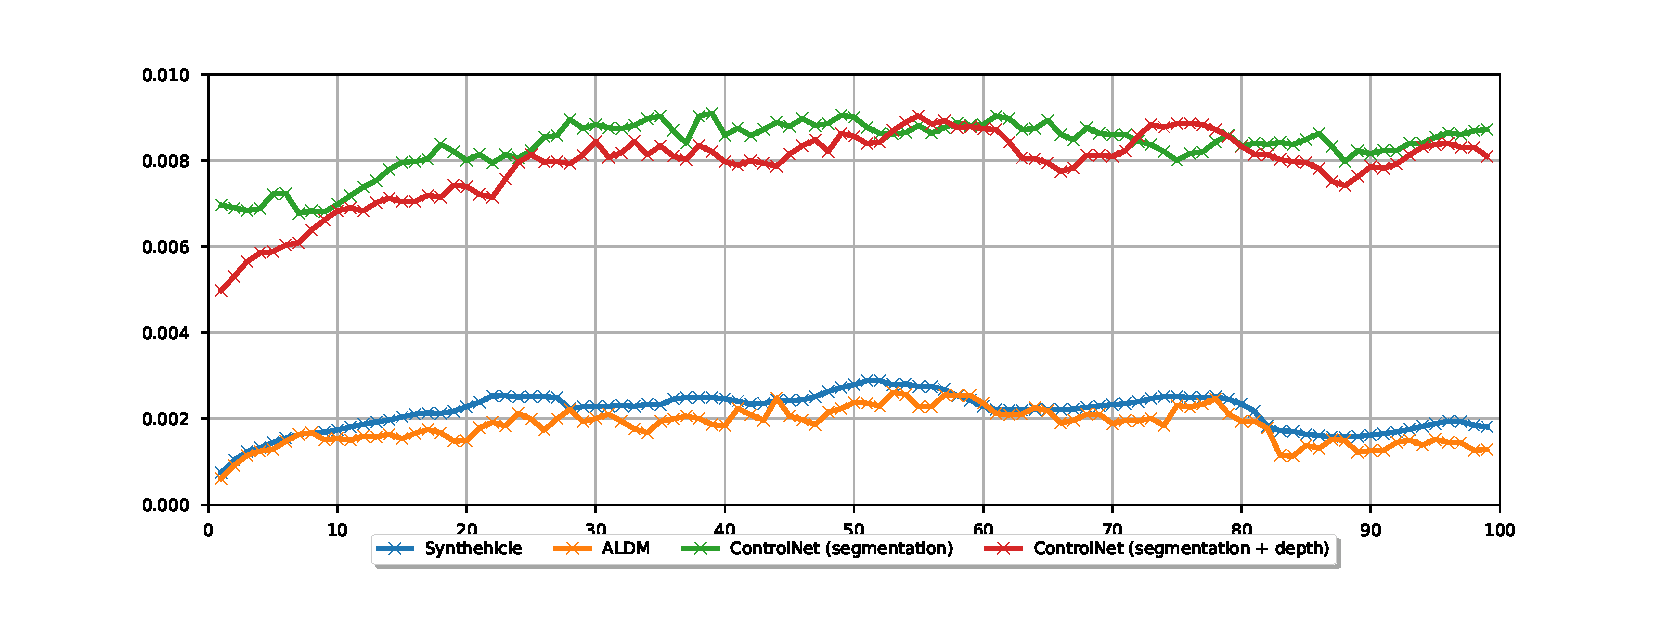
\includegraphics[width=\textwidth]{figures/evaluation/plot_rmse.pdf}
  \caption{RMSE between two following frames. Nearer to the Sythehicle baseline video means better consistency between two frames.}
  \label{fig:rmse_video}
  \clearpage
\end{figure}

\begin{table}[H]
\centering
\small
    \begin{tabular}{lLLLLRL}
    \toprule
          
    Video & \text{Syntheticle} & \text{ALDM} & \text{I2I ControlNet (seg)} &  \multicolumn{2}{c}{I2I ControlNet (seg + depth)}  \\
    \midrule
    Scene 1 & 7     & \textbf{18}   & 36    & 24            \\
    Scene 2 & 15    & \textbf{20}   & 29    & 22            \\
    Scene 3 & 2     & \textbf{4}    & 14    & \textbf{4}    \\
    Scene 4 & 8     & \textbf{8}    & 23    & 24            \\
    Scene 5 & 8     & \textbf{7}    & 63    & 13            \\
    Scene 6 & 9     & 15            & -     & \textbf{14}   \\
        \midrule
    Avg     & 8.2  & \textbf{12.0}  & -      & 16.8   \\
    Avg -1  & 8.2  & \textbf{10.2}  & 29     & 14   \\
    \bottomrule
    \end{tabular}%
    \caption{Results of object detection tests running on the six scenes. The original video marks the baseline. Avg -1 describes the average of all results, but the baseline score replaces the worst score of a generation method.}
    \label{tab:results_object_tracking}  
\end{table}%

\subsubsection{ALDM}
As the test results show, using ALDM for generation yields results that are nearly equivalent to the original video in terms of image stability as well as in the object detection tests. As depicted in \autoref{fig:rmse_video}, the ALDM model dominates the other approaches regarding RMSE between the following frames, showing how stable the images are. Compared to the original video, the RMSE is almost equal. Looking through the videos, spatial consistency is broken at two things: lightning and cars. Especially the cars, the only moving element in the videos, cannot persist in color or shape, even when the same seed is used. This comes with no surprise because of the change in the segmentation map; different pixels are now denoised to generate the cars, leading to other cars. Also, this approach lacks information from the previous frames, making feature-sharing impossible. This also partially explains the gap between the baseline video from Synthehicle and ALDM in the object detection results \autoref{tab:results_object_tracking}. Another problem with ALDM discussed earlier as well, is its training on first-person view data, making it extra hard for the model to generate realistic shapes for the cars from a third-person perspective.

For special constancy, the videos generated by ALDM follow the underlying segmentations and, therefore, are fully consistent with the ground truth.

\begin{figure}[H]
  \centering
  \includegraphics[width=\textwidth]{figures/evaluation/video_analysis.pdf}
  \caption{Frames 21-24 of Scene 1. From top row to bottom row:
synthetic data from Synthehicle, Output ALDM, Output I2I Seg, Output I2I Seg + Depth. The red boxes mark where a pedestrian can be seen clearly.}
  \label{fig:video_analysis}
  \clearpage
\end{figure}

\subsubsection{Image-to-Image with the Segmentation ControlNet}
Looking at the RMSE, image-to-image with a segmentation ControlNet overall performs the worst out of all tested approaches. The information from the previous image combined with the segmentation is too little information to obtain a consistent background, resulting in new generations in each frame.

This is especially bad for the car generation because, together with the prompt, objects that are distorted by previous generations are often converted to cars, resulting in really bad performance in object tracking.

\subsubsection{Image-to-Image with the Depth and Segmentation ControlNet}
For the depth images, it is important to notice how much better details are captured during generation. Looking at the person in Scene 1 \autoref{fig:video_analysis}, in contrast to generation only with the segmentation map, the person is visible and moving correctly. 

This behavior is also captured by the object tracking test. While the depth map does not help that much with maintaining a stable image (see \autoref{fig:rmse_video}), the performance for car tracking drastically improves over the ControlNet with segmentation, sometimes getting even closer to the original Syntehicle video than ALDM.


\subsection{Discussion: Spatial-temporal image consistency}
ALDM dominates in this area with its capabilities to maintain a very good spatial and temporal consistency, while the image-to-image approaches fall short of expectations. Particularly noteworthy here is the preservation of the background, which is almost identical to the previous image. However, it is important to note that all these attempts are based on still cameras. This means that the same noise remains in the same place, which makes it much easier to keep the background stable. With a static camera, it should also be possible to transfer the properties of the moving objects to the subsequent frames with relatively little effort and thus make the cars consistent. With a moving camera, ALDM would have to be fundamentally modified. An example of how this could work would be the \href{https://huggingface.co/CiaraRowles/TemporalNet}{TemporalNet}, which can generate the subsequent frame for another frame by being trained on time series data. Even if the presented results have strong artifacts, TemporalNet's outputs are much more stable than Stable Diffusion outputs. Another possibility would be to go the way of OpenAI Sora  \cite{liu2024sorareviewbackgroundtechnology}, which trains its entire model on time series and outputs its result at once and not iteratively. The problem with Sora's approach is the high training cost, long training time, and low data availability.  